\documentclass{standalone}
\usepackage{tikz}
\usetikzlibrary{patterns, positioning}
\usepackage[sfdefault]{ClearSans} %% option 'sfdefault' activates Clear Sans as the default text font
\usepackage[T1]{fontenc}

\begin{document}
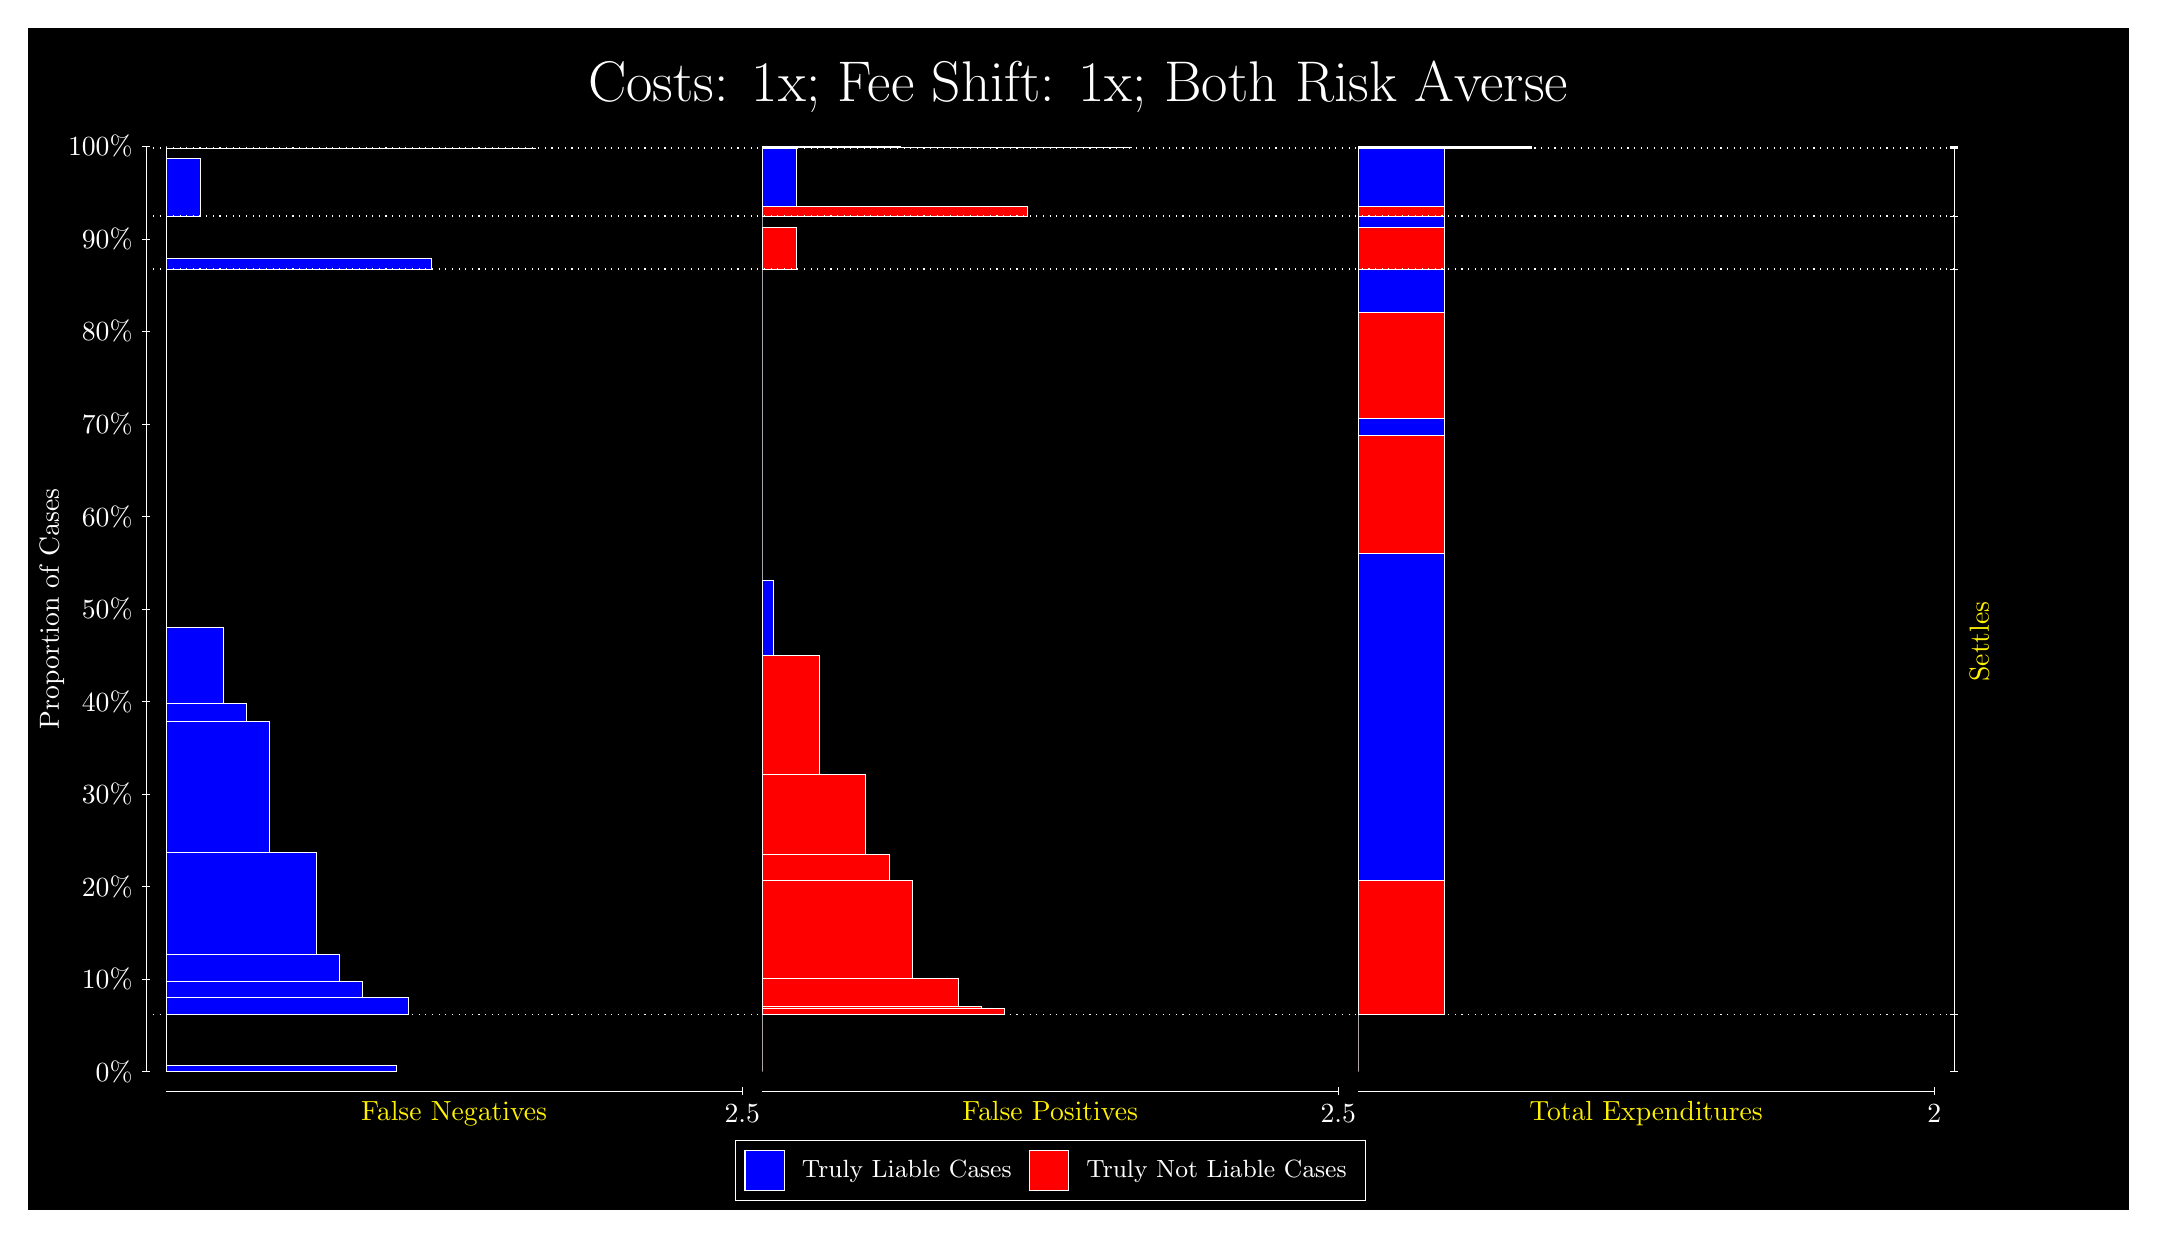
\begin{tikzpicture}
\draw[fill=black] (0,0) rectangle (26.667,15);
\draw[text=white] (0,13.5) rectangle (26.667,15) node[midway] {\huge Costs: 1x; Fee Shift: 1x; Both Risk Averse};
\draw[white, very thin] (1.5,1.75) -- (1.5,13.5);
\node[rotate=90, text=white, anchor=center] at (0.3, 7.625) {Proportion of Cases};
\draw[white, very thin] (1.45,1.75) -- (1.55,1.75);
\node[text=white, anchor=east] at (1.45, 1.75) {0\%};
\draw[white, very thin] (1.45,2.925) -- (1.55,2.925);
\node[text=white, anchor=east] at (1.45, 2.925) {10\%};
\draw[white, very thin] (1.45,4.1) -- (1.55,4.1);
\node[text=white, anchor=east] at (1.45, 4.1) {20\%};
\draw[white, very thin] (1.45,5.275) -- (1.55,5.275);
\node[text=white, anchor=east] at (1.45, 5.275) {30\%};
\draw[white, very thin] (1.45,6.45) -- (1.55,6.45);
\node[text=white, anchor=east] at (1.45, 6.45) {40\%};
\draw[white, very thin] (1.45,7.625) -- (1.55,7.625);
\node[text=white, anchor=east] at (1.45, 7.625) {50\%};
\draw[white, very thin] (1.45,8.8) -- (1.55,8.8);
\node[text=white, anchor=east] at (1.45, 8.8) {60\%};
\draw[white, very thin] (1.45,9.975) -- (1.55,9.975);
\node[text=white, anchor=east] at (1.45, 9.975) {70\%};
\draw[white, very thin] (1.45,11.15) -- (1.55,11.15);
\node[text=white, anchor=east] at (1.45, 11.15) {80\%};
\draw[white, very thin] (1.45,12.325) -- (1.55,12.325);
\node[text=white, anchor=east] at (1.45, 12.325) {90\%};
\draw[white, very thin] (1.45,13.5) -- (1.55,13.5);
\node[text=white, anchor=east] at (1.45, 13.5) {100\%};

\draw[white, very thin] (24.457,1.75) -- (24.457,13.5);
\draw[white, very thin] (24.407,1.75) -- (24.507,1.75);
\node[anchor=west] at (24.407, 1.75) {};
\draw[white, very thin] (24.407,2.4788) -- (24.507,2.4788);
\node[anchor=west] at (24.407, 2.4788) {};
\draw[white, very thin] (24.407,11.942) -- (24.507,11.942);
\node[anchor=west] at (24.407, 11.942) {};
\draw[white, very thin] (24.407,12.615) -- (24.507,12.615);
\node[anchor=west] at (24.407, 12.615) {};
\draw[white, very thin] (24.407,13.474) -- (24.507,13.474);
\node[anchor=west] at (24.407, 13.474) {};
\draw[white, very thin] (24.407,13.485) -- (24.507,13.485);
\node[anchor=west] at (24.407, 13.485) {};
\draw[white, very thin] (24.407,13.5) -- (24.507,13.5);
\node[anchor=west] at (24.407, 13.5) {};

\draw[white, very thin, fill=blue] (1.75,1.75) rectangle (4.6775,1.8267);
\draw[white, very thin, fill=red] (1.75,1.8267) rectangle (1.75,2.4788);
\draw[white, very thin, fill=blue] (1.75,2.4788) rectangle (4.8239,2.6875);
\draw[white, very thin, fill=blue] (1.75,2.6875) rectangle (4.2384,2.8901);
\draw[white, very thin, fill=blue] (1.75,2.8901) rectangle (3.9457,3.2369);
\draw[white, very thin, fill=blue] (1.75,3.2369) rectangle (3.6529,4.5374);
\draw[white, very thin, fill=blue] (1.75,4.5374) rectangle (3.0674,6.2012);
\draw[white, very thin, fill=blue] (1.75,6.2012) rectangle (2.7746,6.4293);
\draw[white, very thin, fill=blue] (1.75,6.4293) rectangle (2.4819,7.3872);
\draw[white, very thin, fill=red] (1.75,7.3872) rectangle (1.75,11.942);
\draw[white, very thin, fill=blue] (1.75,11.942) rectangle (5.1167,12.082);
\draw[white, very thin, fill=red] (1.75,12.082) rectangle (1.75,12.615);
\draw[white, very thin, fill=blue] (1.75,12.615) rectangle (2.1891,13.351);
\draw[white, very thin, fill=red] (1.75,13.351) rectangle (1.75,13.474);
\draw[white, very thin, fill=blue] (1.75,13.474) rectangle (6.4341,13.479);
\draw[white, very thin, fill=red] (1.75,13.479) rectangle (1.75,13.485);
\draw[white, very thin, fill=red] (1.75,13.485) rectangle (1.75,13.489);
\draw[white, very thin, fill=blue] (1.75,13.489) rectangle (1.75,13.5);
\draw[white, very thin, fill=red] (9.3189,1.75) rectangle (9.3189,2.4021);
\draw[white, very thin, fill=blue] (9.3189,2.4021) rectangle (9.3189,2.4788);
\draw[white, very thin, fill=red] (9.3189,2.4788) rectangle (12.393,2.5533);
\draw[white, very thin, fill=red] (9.3189,2.5533) rectangle (12.1,2.5754);
\draw[white, very thin, fill=red] (9.3189,2.5754) rectangle (11.807,2.9282);
\draw[white, very thin, fill=red] (9.3189,2.9282) rectangle (11.222,4.181);
\draw[white, very thin, fill=red] (9.3189,4.181) rectangle (10.929,4.5058);
\draw[white, very thin, fill=red] (9.3189,4.5058) rectangle (10.636,5.5314);
\draw[white, very thin, fill=red] (9.3189,5.5314) rectangle (10.051,7.0336);
\draw[white, very thin, fill=blue] (9.3189,7.0336) rectangle (9.4652,7.9915);
\draw[white, very thin, fill=blue] (9.3189,7.9915) rectangle (9.3189,11.942);
\draw[white, very thin, fill=red] (9.3189,11.942) rectangle (9.758,12.476);
\draw[white, very thin, fill=blue] (9.3189,12.476) rectangle (9.3189,12.615);
\draw[white, very thin, fill=red] (9.3189,12.615) rectangle (12.686,12.739);
\draw[white, very thin, fill=blue] (9.3189,12.739) rectangle (9.758,13.474);
\draw[white, very thin, fill=red] (9.3189,13.474) rectangle (9.3189,13.48);
\draw[white, very thin, fill=blue] (9.3189,13.48) rectangle (9.3189,13.485);
\draw[white, very thin, fill=red] (9.3189,13.485) rectangle (14.003,13.489);
\draw[white, very thin, fill=blue] (9.3189,13.489) rectangle (11.075,13.5);
\draw[white, very thin, fill=red] (16.888,1.75) rectangle (16.888,2.4021);
\draw[white, very thin, fill=blue] (16.888,2.4021) rectangle (16.888,2.4788);
\draw[white, very thin, fill=red] (16.888,2.4788) rectangle (17.986,4.181);
\draw[white, very thin, fill=blue] (16.888,4.181) rectangle (17.986,8.3313);
\draw[white, very thin, fill=red] (16.888,8.3313) rectangle (17.986,9.8335);
\draw[white, very thin, fill=blue] (16.888,9.8335) rectangle (17.986,10.042);
\draw[white, very thin, fill=red] (16.888,10.042) rectangle (17.986,11.393);
\draw[white, very thin, fill=blue] (16.888,11.393) rectangle (17.986,11.942);
\draw[white, very thin, fill=red] (16.888,11.942) rectangle (17.986,12.476);
\draw[white, very thin, fill=blue] (16.888,12.476) rectangle (17.986,12.615);
\draw[white, very thin, fill=red] (16.888,12.615) rectangle (17.986,12.739);
\draw[white, very thin, fill=blue] (16.888,12.739) rectangle (17.986,13.474);
\draw[white, very thin, fill=red] (16.888,13.474) rectangle (19.083,13.48);
\draw[white, very thin, fill=blue] (16.888,13.48) rectangle (19.083,13.485);
\draw[white, very thin, fill=red] (16.888,13.485) rectangle (19.083,13.489);
\draw[white, very thin, fill=blue] (16.888,13.489) rectangle (19.083,13.5);
\draw[white, dotted] (1.5,2.4788) -- (24.457,2.4788);
\draw[white, dotted] (1.5,11.942) -- (24.457,11.942);
\draw[white, dotted] (1.5,12.615) -- (24.457,12.615);
\draw[white, dotted] (1.5,13.474) -- (24.457,13.474);
\draw[white, dotted] (1.5,13.485) -- (24.457,13.485);
\draw[white, very thin] (1.75,1.5) -- (9.0689,1.5);
\node[text=yellow, anchor=north] at (5.4094, 1.5) {False Negatives};
\draw[white, very thin] (9.0689,1.45) -- (9.0689,1.55);
\node[text=white, anchor=north] at (9.0689, 1.45) {2.5};

\draw[white, very thin] (9.3189,1.5) -- (16.638,1.5);
\node[text=yellow, anchor=north] at (12.978, 1.5) {False Positives};
\draw[white, very thin] (16.638,1.45) -- (16.638,1.55);
\node[text=white, anchor=north] at (16.638, 1.45) {2.5};

\draw[white, very thin] (16.888,1.5) -- (24.207,1.5);
\node[text=yellow, anchor=north] at (20.547, 1.5) {Total Expenditures};
\draw[white, very thin] (24.207,1.45) -- (24.207,1.55);
\node[text=white, anchor=north] at (24.207, 1.45) {2};


\node[text=yellow, centered, rotate=90] at (24.777, 7.2104) {Settles};





\draw (12.978300999999998,1.5) node[draw=none] (baseCoordinate) {};
\begin{scope}[align=center]
        \matrix[scale=0.5, draw=white, below=0.5cm of baseCoordinate, nodes={draw}, column sep=0.1cm]{
            \node[rectangle, draw, minimum width=0.5cm, minimum height=0.5cm, fill=blue] {}; &
            \node[draw=none, font=\small, text=white] (B) {Truly Liable Cases}; &
            \node[rectangle, draw, minimum width=0.5cm, minimum height=0.5cm, fill=red] {}; &
            \node[draw=none, font=\small, text=white] (B) {Truly Not Liable Cases}; \\
            };
\end{scope}

\end{tikzpicture}
\end{document}